\documentclass[../main.tex]{subfiles}
\chapter{Herleitung}
\label{c:herleitung}

\section[Operatoren]{Operatoren für Transformationen}
\subsection{Translation}
\begin{equation}
	T_{\mathbf{v}} \begin{pmatrix}t_x\\t_y\\t_z\\\end{pmatrix}= \begin{bmatrix}1 & 0 & 0 & t_x\\0 & 1 & 0 & t_y\\0 & 0 & 0 & t_z\\0 & 0 & 0 & 1\end{bmatrix}
\end{equation}

\subsection{Rotation}
\begin{equation}
	\begin{split}
		R\begin{pmatrix}\gamma\\\beta\\\alpha\\\end{pmatrix} = & R_{z}(\alpha )\,R_{y}(\beta )\,R_{x}(\gamma ) \\
		= & \begin{bmatrix}\cos \alpha & -\sin \alpha & 0\\\sin \alpha & \cos \alpha & 0\\0& 0& 1\\\end{bmatrix}
			\begin{bmatrix}\cos \beta & 0& \sin \beta \\0& 1& 0\\-\sin \beta & 0& \cos \beta \\\end{bmatrix}
			\begin{bmatrix}1& 0& 0\\0& \cos \gamma & -\sin \gamma \\0& \sin \gamma & \cos \gamma \\\end{bmatrix} \\
		= & \begin{bmatrix}
			\cos \alpha \cos \beta & \cos \alpha \sin \beta \sin \gamma -\sin \alpha \cos \gamma & \cos 	\alpha \sin \beta \cos \gamma +\sin \alpha \sin \gamma \\
			\sin \alpha \cos \beta & \sin \alpha \sin \beta \sin \gamma +\cos \alpha \cos \gamma & \sin \alpha \sin \beta \cos \gamma -\cos \alpha \sin \gamma \\
			-\sin \beta & \cos \beta \sin \gamma & \cos \beta \cos \gamma \\
		\end{bmatrix}
	\end{split}
\end{equation}

Um Matrixoperation zu vereinfachen werden Rotationsmatrizen als homogene Transformationsmatrizen gemäß \ref{eq:homTM} mit einem Nullvektor $\mathbf{p} = \mathbf{0}$ als Verschiebung geschrieben.

\subsection[Transformationsmatrix]{Homogene Transformationsmatrix}
Die Anordnung eines körperfesten Koordinatensystems $\{b\}$ (body-frame) in einem raumfesten Koordinatensystem $\{s\}$ (space-frame) kann beschrieben werden durch die Position des body-frames $p$ in $\{s\}$-Koordinaten und einer Rotationsmatrix $R$, welche die Ausrichtung von $\{b\}$ in $\{s\}$-Koordinaten.

\begin{equation}
	\label{eq:homTM}
	T = \begin{bmatrix}R & p\\0 & 1\end{bmatrix} = \begin{bmatrix}r_{11} & r_{12} & r_{13} & p_1\\r_{21} & r_{22} & r_{23} & p_2\\r_{31} & r_{32} & r_{33} & p_3\\0 & 0 & 0 & 1\end{bmatrix}
\end{equation}

\subsection{Inverse einer Transformationsmatrix}

\begin{equation}
	\begin{split}
		\mathbf{T}^{-1} & = \begin{bmatrix}R & p\\0 & 1\end{bmatrix}^{-1}\\
		& = \begin{bmatrix}R^\intercal & -R^\intercal \cdot p\\0 & 1\end{bmatrix}
	  \end{split}
\end{equation}

Bei einer linearen Translation ist die Rotationsmatrix die Einheitsmatrix. Daher ergibt sich für die Translationskomponente:

\begin{equation}
	\begin{split}
		-R^\intercal \cdot p & = (-1) \cdot \begin{bmatrix}1 & 0 & 0\\0 & 1 & 0\\0 & 0 & 1\end{bmatrix}^\intercal \cdot p\\
							 & = \begin{bmatrix}-1 & 0 & 0\\0 & -1 & 0\\0 & 0 & -1\end{bmatrix} \cdot \begin{pmatrix}t_x\\t_y\\t_z\end{pmatrix}\\
							 & = \begin{pmatrix}-t_x\\-t_y\\-t_z\end{pmatrix}
	\end{split}
\end{equation}

Daher ergibt sich für die Inverse der translatorischen Transformationsmatrix.

\begin{equation}
	T^b_s\begin{pmatrix}t_x\\t_y\\t_z\end{pmatrix}^{-1} = T^s_b\begin{pmatrix}-t_x\\-t_y\\-t_z\end{pmatrix}
\end{equation}

Die Transformsrichtungs-Indizes kehren sich um zu beschreiben, dass die Transformationsrichtung jetzt vom body-frame $\{b\}$ in das space-frame $\{s\}$ erfolgt.

\subsection{Inverse einer Rotationsmatrix um eine Achse}

Beweis oder Quelle!

\begin{equation}
	\left(R_s^b\begin{pmatrix}\gamma\\0\\0\end{pmatrix}\right)^{-1} = R^s_b\begin{pmatrix}-\gamma\\0\\0\end{pmatrix}
\end{equation}

\subsection{Notation der Indizes}

Um bei einer Transformation zu verdeutlichen aus welchem Koordinatensystem in welches andere Koordinatensystem transformiert wird, werden der Transformationsmatrix Indizes angehängt.

\begin{figure}
	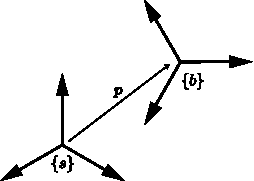
\includegraphics{frames}
	\caption{Transformation von space-frame $\{s\}$ nach body-frame $\{b\}$}
	\label{fig:frames}
\end{figure}

Das Subscript steht dabei für das Ausgangskoordinatensystem, das Superscript steht für die Zielkoordinatensystem. Die zu Abb.\ \ref{fig:frames} gehörende Transformationsmatrix lautet also:

\begin{equation}
	T_s^b = \begin{bmatrix}R_s^b & p\\0 & 1\end{bmatrix}
\end{equation}

\section[Maschine]{Kinematik der Maschine}

Im Folgenden wird die Kinematik der Maschine in Abb.\ \ref{fig:maschine} beschrieben. Die Kinematik wird für die Betrachtung ausgehend von der Schnittstelle Maschinenbett-Werkstück in zwei Bereiche eingeteilt, für welche jeweils die Koordinatentransformation aufgestellt wird. Ein Bereich betrachtet auf Seite des Werkzeugs die kinematische Kette der Maschine mit den verfahrbaren Achsen, der zweite auf der Seite des Werkstücks die Position und Verdrehwinkel des Werkstückkoordinatensystems im Maschinenbett. Um anschließend die Koordinatentransformation von dem Werkzeugkoordinatensystems ind das Werkstückkoordinatensystems zu erhalten, werden die beiden Terme gleichgesetzt und nach Werkzeugkoordinaten aufgelöst.

\begin{figure}
	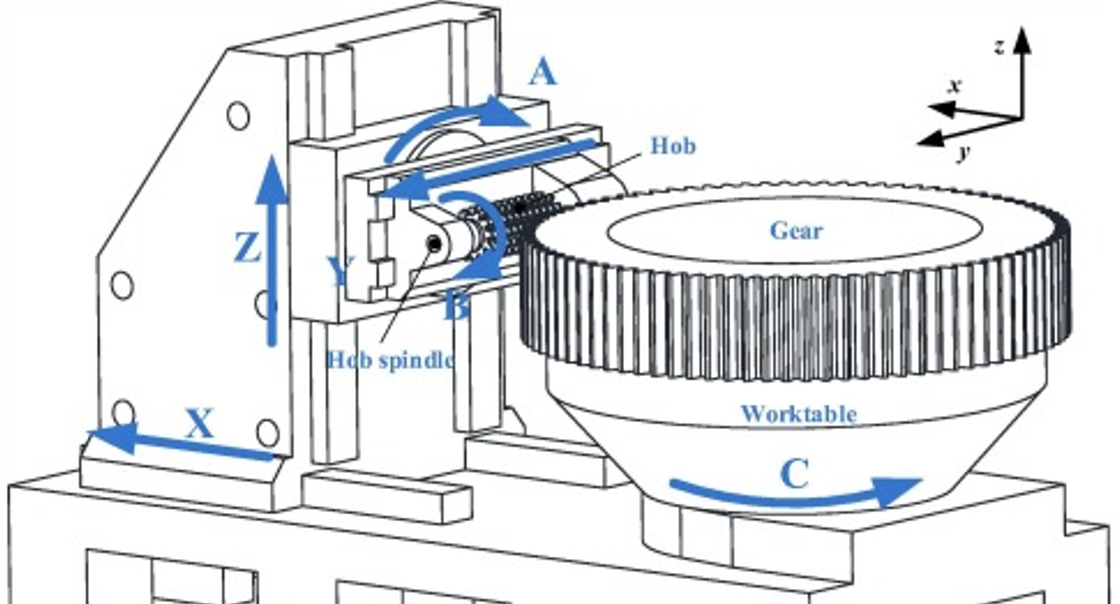
\includegraphics[width=12cm]{maschine_frei}
	\caption{Kinematik der Maschine mit Vorzeichenrichtung der Achsen}
	\label{fig:maschine}
\end{figure}

\subsection[Werkstück]{Kinematik der Werkstück-Seite}

In die kinematische Kette auf der Werkstückseite \ref{eq:werkstuck} gehen ein Offset des Werkstückkoordinatensystems zum Maschinenkoordinatensystem $\mathbf{p}_{offset} = \begin{pmatrix} a\\b\\c\end{pmatrix}$ und der Verdrehwinkel $C$ ein. Der Offset erlaubt die Fähigkeit ein versetztes Aufspannen des Werkstücks darzustellen und ist im idealen Fall ein Nullvektor. Dem Verdrehwinkel wird ein weiterer Offest $\gamma$ aufgeprägt. Dieser stellt den Fehler des verdrehten Aufspannens dar und erlaubt die Position von Zahn und Zahnlücke des virtuellen Schneckengetriebes zu korrigieren.

\begin{equation}
	\label{eq:werkstuck}
	\mathbf{p}_m = T_{\mathbf{v}} \begin{pmatrix}a\\b\\c\\\end{pmatrix} \cdot{} R \begin{pmatrix}0\\0\\C - \gamma\\\end{pmatrix} \cdot{} \mathbf{p}_{WSt}
\end{equation}

Die Transformation beschreibt die Position eines Werkstückpunktes im Koordinatensystems des Maschinenbettes.

\subsection[Werkzeug]{Kinematik der Werkzeug-Seite}

Die kinematische Kette der Werkzeugseite \ref{eq:werkzeug} beinhaltet die verfahrbaren Achsen der Maschine mit ihrem jeweiligen Freiheitsgrad ein. Dabei wird dem y-Achsenfreiheitsgrad ein Offset aufgeprägt, mit dem der Bereich des Werkzeuges im Eingriff verschoben werden kann. Das Werkzeug unterliegt beim Schneiden Verschleiß. Das Werkzeug ist länger als erforderlich und durch Verschieben des Werkzeugs entlang der y-Achse kann der Verschleiß gleichmäßig auf das Werkzeug verteilt werden. Die Drehrichtung des Werkzeuges ist außerdem mathematisch negativ.

\begin{equation}
	\label{eq:werkzeug}
	\mathbf{p}_m = T_{\mathbf{v}} \begin{pmatrix}X\\0\\Z\\\end{pmatrix} \cdot{} R \begin{pmatrix}A\\0\\0\\\end{pmatrix} \cdot{} T_{\mathbf{v}} \begin{pmatrix}0\\Y+s\\0\\\end{pmatrix} \cdot{} R \begin{pmatrix}0\\-B\\0\\\end{pmatrix} \cdot{} \mathbf{p}_{WZ}
\end{equation}

Die Transformation beschreibt die Position eines Werkzeugpunktes im Koordinatensystems des Maschinenbettes.\\
Zur Vereinfachung der entstehenden Terme bietet sich das Zusammenfassen der Transformationsmatrizen zu einer Transformationsmatrix von Maschinenbett- in Werkzeugkoordinaten an:

\begin{equation}
	\mathbf{T}^{WZ}_m = T_{\mathbf{v}} \begin{pmatrix}X\\0\\Z\\\end{pmatrix} \cdot{} R \begin{pmatrix}A\\0\\0\\\end{pmatrix} \cdot{} T_{\mathbf{v}} \begin{pmatrix}0\\Y+s\\0\\\end{pmatrix} \cdot{} R \begin{pmatrix}0\\-B\\0\\\end{pmatrix}
\end{equation}


\subsection[Vorschübe]{Aufprägung der Vorschübe auf die Achskoordinaten}

Durch die Natur der Fertigung von Verzahnung vergleichbar mit einem Schneckengetriebe hängen die Vorschübe der Achsen von der Rotation des Werkzeugs ab. Dazu wird die Abhängigkeit der Achskoordinaten vom Werkzeugwinkel als Produkt des Werkzeugwinkels und einem Vorschubfaktor beschrieben. Den x-Achsen und z-Achsen Koordinaten wird zusätzlich als linearer Offset die Position der x-Achse von einem Ausgangszustand aufgeprägt. Bei der C-Achse ist dieser Effekt bereits mit dem Winkeloffset $\gamma$ realisiert.

\subsubitem{x-Axchse}

\begin{equation}
	X = x + B \cdot fX_{WZ,rad}
\end{equation}

\subsubitem{z-Axchse}

\begin{equation}
	Z = z + B \cdot fZ_{WZ,rad}
\end{equation}

\subsubitem{C-Axchse}

\begin{equation}
	C = B \cdot fC_{WSt,rad}
\end{equation}

Damit ergibt sich für die Transformationsmatrix von Maschinenbett- in Werkzeugkoordinaten:

\begin{equation}
	\mathbf{T}^{WZ}_m = T_{\mathbf{v}} \begin{pmatrix}x + B \cdot fX_{WZ,rad}\\0\\z + B \cdot fZ_{WZ,rad}\\\end{pmatrix} \cdot{} R \begin{pmatrix}A\\0\\0\\\end{pmatrix} \cdot{} T_{\mathbf{v}} \begin{pmatrix}0\\Y+s\\0\\\end{pmatrix} \cdot{} R \begin{pmatrix}0\\-B\\0\\\end{pmatrix}
\end{equation}

\subsection[Gesamt]{Transformation von Werkzeug- in Werkstückkoordinaten}

Um die Transformation aus dem Werkzeug- in das Werkstückkoordinatensystem zu erhalten setzen wir die beiden Transformationsschritte gleich:

\begin{equation}
	T_{\mathbf{v}} \begin{pmatrix}a\\b\\c\\\end{pmatrix} \cdot{} R \begin{pmatrix}0\\0\\C - \gamma\\\end{pmatrix} \cdot{} \mathbf{p}_{WSt}= T_{\mathbf{v}} \begin{pmatrix}X\\0\\Z\\\end{pmatrix} \cdot{} R \begin{pmatrix}A\\0\\0\\\end{pmatrix} \cdot{} T_{\mathbf{v}} \begin{pmatrix}0\\Y+s\\0\\\end{pmatrix} \cdot{} R \begin{pmatrix}0\\-B\\0\\\end{pmatrix} \cdot{} \mathbf{p}_{WZ}
\end{equation}

Die Gleichung wird durch Multiplikation mit den Inversen der Transformation- und Rotationsmatrix aufgelöst, sodass die Beschreibung der Transformation von Werkzeug- in Werkstückkoordinaten entsteht.

\begin{equation}
	 \mathbf{p}_{WSt} = R \begin{pmatrix}0\\0\\-(C - \gamma)\\\end{pmatrix} \cdot{} T_{\mathbf{v}} \begin{pmatrix}-a\\-b\\-c\\\end{pmatrix} \cdot{} T_{\mathbf{v}} \begin{pmatrix}X\\0\\Z\\\end{pmatrix} \cdot{} R \begin{pmatrix}A\\0\\0\\\end{pmatrix} \cdot{} T_{\mathbf{v}} \begin{pmatrix}0\\Y+s\\0\\\end{pmatrix} \cdot{} R \begin{pmatrix}0\\-B\\0\\\end{pmatrix} \cdot{} \mathbf{p}_{WZ}
\end{equation}